
\documentclass[a4paper,UKenglish,cleveref, autoref, thm-restate,authorcolumns]{lipics-v2019}
%This is a template for producing LIPIcs articles. 
%See lipics-manual.pdf for further information.
%for A4 paper format use option "a4paper", for US-letter use option "letterpaper"
%for british hyphenation rules use option "UKenglish", for american hyphenation rules use option "USenglish"
%for section-numbered lemmas etc., use "numberwithinsect"
%for enabling cleveref support, use "cleveref"
%for enabling autoref support, use "autoref"
%for anonymousing the authors (e.g. for double-blind review), add "anonymous"
%for enabling thm-restate support, use "thm-restate"

\usepackage[utf8]{inputenc}
\usepackage{graphicx}
\usepackage{algorithm}
\usepackage[noend]{algpseudocode}
\usepackage{todonotes}
\usepackage{array}

\def\Balph{{\cal B}}% Barcode alphabet
\def\MolOrd{{\cal O}}% Total order on molecules
\def\MolSet{{\cal M}}% Molecules set


\usepackage{amsthm}
%\newtheorem{lemma}{Lemma}
\newtheorem{property}{Property}
%\newtheorem{claim}{Claim}
\newtheorem{conjecture}{Conjecture}
%\newtheorem{remark}{Remark}
\newtheorem{question}{Question}
%\newtheorem{definition}{Definition}
\newtheorem{problem}{Problem}

%\graphicspath{{./graphics/}}%helpful if your graphic files are in another directory

\bibliographystyle{plainurl}% the mandatory bibstyle

\title{A graph-theoretic barcode ordering model for linked-reads}

%\titlerunning{Dummy short title} %TODO optional, please use if title is longer than one line

\author{Yoann Dufresne}{Department of Computational Biology, C3BI USR 3756 CNRS, Institut Pasteur, Paris, France}{yoann.dufresne@pasteur.fr}{https://orcid.org/0000-0002-0930-8920}{}%TODO mandatory, please use full name; only 1 author per \author macro; first two parameters are mandatory, other parameters can be empty. Please provide at least the name of the affiliation and the country. The full address is optional

\author{Chen Sun}{Department of Computer Science and Engineering, The Pennsylvania State University, USA}{chensunx@gmail.com}{}{}

\author{Pierre Marijon}{Center for Bioinformatics, Saarland University, Saarland Informatics Campus E2.1, 66123 Saarbrücken, Germany}{pmarijon@mmci.uni-saarland.de}{https://orcid.org/0000-0002-6694-6873}{}

\author{Dominique Lavenier}{IRISA, Inria, Universit\'e de Rennes, France}{lavenier@irisa.fr}{https://orcid.org/0000-0003-2557-680X}{}

\author{Cedric Chauve}{Department of Mathematics, Simon Fraser University, Canada \and LaBRI, Universit\'e de Bordeaux, France}{cedric.chauve@sfu.ca}{[orcid]}{NSERC Discovery Grant RGPIN-03986}

\author{Rayan Chikhi}{Department of Computational Biology, C3BI USR 3756 CNRS, Institut Pasteur, Paris, France}{rayan.chikhi@pasteur.fr}{https://orcid.org/0000-0003-1099-8735}{INCEPTION project (PIA/ANR-16-CONV-0005)}

\authorrunning{Dufresne \emph{et al}.}

\Copyright{Yoann Dufresne, Pierre Marijon, Cedric Chauve and Rayan Chikhi} %TODO mandatory, please use full first names. LIPIcs license is "CC-BY";  http://creativecommons.org/licenses/by/3.0/

%\ccsdesc[100]{\textcolor{red}{Replace ccsdesc macro with valid one}} %TODO mandatory: Please choose ACM 2012 classifications from https://dl.acm.org/ccs/ccs_flat.cfm 
\begin{CCSXML}
<ccs2012>
   <concept>
       <concept_id>10010405.10010444.10010450</concept_id>
       <concept_desc>Applied computing~Bioinformatics</concept_desc>
       <concept_significance>500</concept_significance>
       </concept>
 </ccs2012>
\end{CCSXML}

\ccsdesc[500]{Applied computing~Bioinformatics}

\keywords{DNA sequencing, graph algorithms, linked-reads, interval graphs, cliques} %TODO mandatory; please add comma-separated list of keywords

\category{} %optional, e.g. invited paper

\relatedversion{} %optional, e.g. full version hosted on arXiv, HAL, or other respository/website
%\relatedversion{A full version of the paper is available at \url{...}.}

\supplement{\url{https://gitlab.pasteur.fr/ydufresne/linkedreadsmoleculeordering}}%optional, e.g. related research data, source code, ... hosted on a repository like zenodo, figshare, GitHub, ...

%\funding{(Optional) general funding statement \dots}%optional, to capture a funding statement, which applies to all authors. Please enter author specific funding statements as fifth argument of the \author macro.

\acknowledgements{The authors are grateful to Paul Medvedev for preliminary work and discussions.}%optional

%\nolinenumbers %uncomment to disable line numbering

%\hideLIPIcs  %uncomment to remove references to LIPIcs series (logo, DOI, ...), e.g. when preparing a pre-final version to be uploaded to arXiv or another public repository

%Editor-only macros:: begin (do not touch as author)%%%%%%%%%%%%%%%%%%%%%%%%%%%%%%%%%%
\EventEditors{John Q. Open and Joan R. Access}
\EventNoEds{2}
\EventLongTitle{42nd Conference on Very Important Topics (CVIT 2016)}
\EventShortTitle{}
\EventAcronym{CVIT}
\EventYear{2016}
\EventDate{December 24--27, 2016}
\EventLocation{Little Whinging, United Kingdom}
\EventLogo{}
\SeriesVolume{42}
\ArticleNo{23}
%%%%%%%%%%%%%%%%%%%%%%%%%%%%%%%%%%%%%%%%%%%%%%%%%%%%%%

\begin{document}

\maketitle

%TODO mandatory: add short abstract of the document
\begin{abstract}
%We consider two theoretical graph problems that originate from modelling linked-read sequencing. The setting is as follows. 
Considering a set of intervals on the real line, an interval graph records these intervals as nodes and their intersections as edges. Identifying (i.e. merging) pairs of nodes in an interval graph results in a multiple-interval graph. 
%One can then glue pairs of nodes (discarding any edge between a pair of glued nodes) to form a multiple-interval graph. 
Given only the nodes and the edges of the multiple-interval graph without knowing the underlying intervals, we are interested in the following questions. Can one determine how many intervals correspond to each node? Can one compute a walk over the multiple-interval graph nodes that reflects the ordering of the original intervals? These questions are closely related to linked-read DNA sequencing, where barcodes identify long molecules (our intervals) whose intersection graph forms an interval graph. %which are then sequenced using short reads. A sequence barcode is attached to each short read for the identification of its originating molecule, 
Each barcode may correspond to multiple molecules, which complicates downstream analysis, and correspond to the identification of nodes of the corresponding interval graph. % such as de novo assembly. %while this generally does not pose an issue when a reference genome is available, it complicates downstream reference-free analysis such as de novo assembly. 
Resolving the above graph-theoretic problems would facilitate analyses of linked-reads sequencing data, through enabling the conceptual separation of barcodes into molecules and providing, through the molecules order, a skeleton for assembling accurately sequenced reads. Here, we propose a framework that takes as input an arbitrary intersection graph (such as an overlap graph of barcodes) and constructs a heuristic approximation of the ordering of the original intervals.
\end{abstract}

\section{Introduction}
\label{sec:introduction}

%\footnote{This intro has paragraphs that were partly written by Paul, hope he'll be okay with it}
A well-known limitation of short-read sequencing is that it does not provide long-range information, which is crucial to many biological endeavors, such as genome assembly and structural variant identification.
There have been several sequencing technologies developed to overcome this limitation, such as matepair libraries, Hi-C, and long reads (PacBio \& Oxford Nanopore).
Another family of approaches is linked-read sequencing, which includes 10XGenomics Chromium, stLFR~\cite{Wang2019}, CPTv2-seq~\cite{Zhang2017} and TELL-seq~\cite{Chen2019}.
In these approaches, DNA is cloned and cut into large molecules (10-100 kbp), which are then isolated (physically in 10X, or virtually by the others using beads) % in the same tube) 
and sheared into shorter fragments. A barcode is attached to each short fragment for identification of its originating molecule.
Importantly, barcodes do not uniquely identify molecules: several molecules are typically labeled with the same barcode.
The number of different barcodes differ from 150k for CPTv2 to 2 billions for TELL-seq.
Fragments are then sequenced using a standard short-read protocol (e.g Illumina).


Linked-reads have been used to assemble genomes~\cite{supernova}, detect complex structural variants~\cite{greer2017linked}, and more
recently assemble metagenomes~\cite{athena}. A common challenge faced by most linked-read methods is that in order
to make use of the linking information, the reads within each barcode should be first separated into their
constituent molecules. 
%The molecule separation problem is to replace the barcode identifiers of each read with a molecule identifier. 
More formally, for each read $r$, we would like to find the identifier $mi(r)$ of its
originating molecule, given as input an observed identifier $b(mi(r))$, where $b(x)$ associates a barcode identifier
to a molecule $x$. Note that the image of $b$ (all barcodes) is significantly smaller than its domain (all molecules),
hence $b$ can be viewed as a non-invertible hash function. Currently, this problem is being tackled, one way
or another, as part of any method using linked-read data. 
% Cedric: enleve car ca met trop de focus sur la separation de molecules
%However, formulating and solving this as an independent problem can allow downstream methods to focus on their respective tasks, while assuming that the reads have already been separated into molecules. 
%
%Finding overlaps between reads sharing two barcodes can also be framed as the detection of overlaps between the underlying molecules. 
Switching from a read-centric %or barcode-centric 
view to a molecule-centric view opens the possibility of using  methodology similar to long-read overlap graphs. Finding an ordering of barcodes that reflects the underlying order of molecules would indeed greatly facilitate and decrease errors during the scaffolding stage of genome assembly. As noted by the authors of the ARCS scaffolder~\cite{arcs}, different molecules having the same barcode can induce false joins in a scaffolding algorithm, resulting in misassemblies.

Observe that linked-read mapping tools such as \texttt{longranger} or \texttt{ema}~\cite{ema} are able to infer molecules by clustering mapping locations of reads from the same barcode. 
While such reference-based algorithms are often applicable, they do not replace the need for \emph{de novo} algorithms. The quality of reference-based algorithms is related to the quality of the assembly, since clusters cannot be identified across across different contigs. When the genome or metagenome references are in a draft state, molecules will frequently span multiple contigs, preventing their identification. Moreover, in many situations the reference is simply unavailable.

To the best of our knowledge, the barcode ordering problem has not been previously studied, and the assignment of molecule identifiers to reads without a reference has only been previously studied in~\cite{minerva}, where it was referred to as
\emph{barcode deconvolution}. The authors first constructed a bipartite graph between reads and barcodes. An edge $(r, b)$ was added when a k-mer of read $r$ was found in another read of barcode $b$. Then a second graph was constructed with reads as nodes, and edges indicating whether two reads were connected to sufficiently many common barcodes in the bipartite graph. Finally, the second graph was clustered and each cluster reflected reads from the same molecule. This algorithm was implemented in a single-threaded Python language prototype, \texttt{Minerva}. We note that Minerva only assigns molecules identifiers to a fraction of the reads. In our tests on a simulated \emph{E. coli} dataset, Minerva reported results for 12\% of the reads, inferring around 50\% of the true number of molecules.

This raises the question of whether reference-free inference of molecules is fundamentally unsolvable in the setting of linked-read data, or whether an adequate technique has just not yet been found. Surely there exist corner cases where the problem is either impossible, e.g. in an hypothetical situation where all molecules are assigned to the same barcode, or trivial, when each molecule is assigned to a different barcode. As we will see in Section 2, while there exist previous works in graph theory (e.g. in a setting corresponding to all barcodes containing just 2 molecules), the general setting does not appear to have previously been studied.

% Rayan: we perhaps don't need to develop limitations of Minerva in here anymore
% An important limitation of \texttt{Minerva} is that its main data structure (the bipartite read-barcode graph) requires $O(n)$ memory, where $n$ is the number of reads. This is impractical for datasets with hundreds of millions or billions of reads. Also, \texttt{Minerva} only uses shared k-mers between reads, and may fail to identify a molecule if an insufficient number of reads share k-mers with reads from other molecules.

In this paper, we establish theoretical grounds for studying the feasibility of inferring molecule without a reference genome. %We also provide a different resolution approach than the one proposed in \texttt{Minerva}, as 
We will not directly tackle the problem of assigning molecule identifiers to reads (as Minerva does), but instead we look at two problems which can be reduced, in the complexity sense, to molecule inference: %(detailed later in Section 1.1): 
\begin{enumerate}
    \item \textbf{Molecule counting}: count the number of molecules assigned to each barcode
    \item \textbf{Molecule ordering}: reconstruct a total (or partial) order of molecules as a sequence of barcodes
\end{enumerate}
Staying at the level of barcodes and molecules instead of reads will allow to thoroughly establish expectations on whether molecule inference is at all feasible, %Indeed, if one can solve molecule inference, then those two sub-problems can directly be solved; taking the contraposite [..] % I don't know how to finish this sentence 
and how various parameters (e.g. number of molecules, how many molecules per barcode, etc) influence its difficulty. 

We first present the commononalities between the barcodes ordering problem, and the previously-known concepts of interval graphs and multiple-intervals graphs. We then introduce a novel object, the barcode graph, which models overlaps between  the molecules across different barcodes.
By identifying maximal cliques in the barcode graph, which are then paired into structures that we call local clique-pairs, we show that we can construct an auxiliary graph %, the local clique-pairs graph, 
that captures a strong signal related to the ordering of the barcodes according to their underlying molecules.
We apply this technique to synthetic interval graphs, as well as barcode graphs constructed from simulated molecules from a real genome, and show that we are able to accurately count the number of molecules per barcode, and reconstruct an approximate but accurate molecule ordering on barcodes. Finally, we demonstrate how to construct a barcode graph directly from linked-read sequencing data.


%This paper will focus on the first two problems because answering them can be the first step prior to any clustering approach.
%Minerva solves question 3 (to which an answer to question 1 can be derived) but not 2. In this article, we will focus on questions 1 and 2.

%%%%%%%%%%%%%%%%%%%%%%%%%%%%%%%%%%%%%%%%%%%%%%%%%%%%%%%%%%%%%%%%%%%%%%%%%%%
\section{Models and Methods}
\label{sec:methods}

We consider the problem of sequencing a single long DNA molecule (e.g. a chromosome) using linked reads. 
We first introduce the notion of barcode graph, discuss its link with well-known graph classes leading to the conclusion that solving the molecules ordering problem for a barcode graph is likely difficult. 
Next we introduce another graph structure, the local clique-pairs graph, inspired of approaches used to realise an interval graph.

We assume that the sequencing data were obtained by sequencing $n$ fragments (called \textit{molecules} from now) from the chromosome, each molecule being assigned a barcode, where several molecules can be assigned the same barcode; for a molecule $m$ we denote by $b(m)$ its barcode.
We denote by $\Balph{}$ the barcode alphabet and by $|\Balph|=m$ its size, i.e. the total number of observed barcodes; for a barcode $b$ we denote by $m(b)$ the molecules it labels (the barcode size). Let $F = \max_{b\in \Balph} |m(b)|$.
Finally, we assume that no two molecules do start at the same coordinate, which implies that molecules can be totally ordered by their start coordinates.

% -----------------------------------------------------------------------------------------
\subsection{Barcode graphs and families of interval graphs. \label{sec:interval_graph}}
\label{ssec:barcode_graphs}

The sequenced molecules can be seen as intervals along the real line if the sequenced chromosome is linear, or arcs around a circle if it is circular; their \textit{intersection graph} is the graph whose vertices are the $n$ molecules and two vertices are linked by an edge if the corresponding intervals do intersect. 
Intersection graphs of intervals on the real line (resp. arcs around a circle) form the class of \textit{interval graphs} (resp. \textit{circular-arc graphs}).
It is well-known that deciding if a graph is an interval graph or an arc-circular graph can be done in linear time~\cite{BoothL_1976,McConnell_2003}, and many algorithmic problems that are computationally hard in general graphs are tractable in these graph classes~\cite{Golumbic_2004}.

However, the result of the sequencing experiment with linked reads does not provide direct knowledge of the sequenced molecules and of their intersections, as the reads originating from molecules having the same barcode $b$ are all labeled by $b$ and, as discussed in introduction, the problem of separating reads with the same barcodes into cluster corresponding to molecules is non-trivial.
Nevertheless, we assume here first that it is possible to infer, from the barcoded reads if, for a given pair of barcodes $b_1,b_2$ there exists molecules  $m_1$ and $m_2$ such that $b(m_1)=b_1$, $b(m_2)=b_2$ and  and $m_1$ and $m_2$ do intersect: we then say that barcodes $b_1$ and $b_2$ do \textit{intersect}. 
We assume here moreover that we do not observe two intersecting molecules $m_1$ and $m_2$ such that $b(m_1)=b(m_2)$\footnote{We justify this assumption as such molecules could be seen as a single molecule defined by the union of $m_1$ and $m_2$; moreover, simulations with realistic sequencing parameters show that this situation occurs rarely and most often with molecules that share a small intersection.}.

\begin{definition}
    \label{def:barcode_graph}
    The \textit{exact barcode graph} of a set of barcoded molecules is the graph with vertex set $\Balph{}$ and edges between pairs of intersecting barcodes. 
\end{definition}

In the case of a linear chromosome, exact barcode graphs generalize the class of interval graphs and form another well-studied graphs class, \textit{multiple-interval graphs}~\cite{FellowsHRV_2009}. 
Moreover if we assume that each barcode labels exactly $f$ molecules, exact  barcode graphs form the class of $f$-interval graphs; finally, under the additional assumption that all sequenced molecules have exactly the same length, exact barcode graphs are equivalent to the class of \textit{unit $f$-interval graph}. 
We are not aware of any study of the equivalent graph classes for circular chromosomes, i.e. arcs around a circle, and from now on we concentrate on the case of linear chromosomes.
We describe below the formulation of several algorithmic problems related to barcode graphs and how they translate into problems on the aforementioned graph classes.
Note that an exact barcode graph can be a multi-graph in the case where there exists molecules $m_1,m_2,m_3,m_4$ with $b(m_1)=b(m_3)$, $b(m_2)=b(m_4)$ and $m_1,m_2$ (resp. $m_3,m_4$) do intersect.

\smallskip\noindent\textit{Recognizing exact barcode graphs.}
The link with unit $f$-interval graph, although it assumes an unrealistic uniformity in the sequencing process (uniform molecules length and uniform number of molecules per barcode) sheds a light on the computational hardness of analyzing barcoded sequencing data. 
Indeed, recognizing $2$-interval graphs is NP-complete~\cite{WestS_1984}, while the complexity of recognizing unit $f$-interval graphs is still open,  the only positive recognition result being for depth-2 unit $f$-interval graphs~\cite{Jiang_2013}, corresponding to the case where no chromosome base is covered by more than two molecules, an unrealistic assumption for sequencing experiments. 
To the best of our knowledge, given a graph on a barcode alphabet whose edges represent possible molecules intersections, deciding if it is an exact barcode graph, even in the setting of molecules of uniform length and barcodes of uniform size, is open.

%Also, many optimization problems are tractable in interval graphs but intractable in multiple-interval graphs~\cite{ButmanHLR_2007,FellowsHRV_2009}.
\smallskip\noindent\textit{Realizing an exact barcode graph.}
A barcode sequence is a sequence $b_1 \dots b_n$ over the barcode alphabet. 
Given a barcode graph $BG$, a barcode sequence \textit{realizes} $BG$ if every edge of $BG$ can be assigned to two barcodes of the sequence in such a way that if $b_j$ is covered by an edge between $b_i$ and $b_k$ (i.e. $i<j<k$) then there are also edges between $b_i$ and $b_j$ and between $b_j$ and $b_k$.
The molecules ordering problem applied to an exact barcode graph $BG$ is then equivalent to finding a barcode sequence realizing $BG$. 
This problem is tractable in the case of interval graphs ($F=1$); note that if intervals lengths are also fixed, then the problem becomes NP-complete~\cite{PeerS_1997}, while it solvable in polynomial time if additionally the intersection lengths are provided~\cite{KoblerKW_2015}.
We are not aware of similar tractability results for multiple-interval graphs.
However, existing algorithms to realize interval graphs are mainly based on the property that such a realization can be obtained by a sequence of overlapping maximal cliques.
While maximal cliques are easy to find in an interval graph, it is not the case in multiple-interval graph, as the problem of finding the maximum clique in multiple-interval graphs is NP-complete, even for unit $2$-interval graphs~\cite{FrancisGO_2015}, although approximation and parameterized algorithms do exist~\cite{ButmanHLR_2007,FellowsHRV_2009}.
Moreover a structural property of interval graphs that is important toward the realization through maximal cliques, the existence of a vertex whose neighborhood is a clique, does not hold for multiple interval graphs~\cite{Bar-YehudaHNSS_2006}.
Finally, it is easy to see that a maximal cliques of size $c$ in an exact barcode graph might not correspond to a set of $c$ pairwise intersecting molecules.
This leads us to conjecture that realizing an exact barcode graph is difficult.

\smallskip\noindent\textit{Handling inexact barcode graphs.}
Constructing an exact barcode graph implies to detect intersecting barcodes from sequenced barcoded reads and it is thus likely unrealistic to expect perfectly obtaining such a graph from sequencing data. 
It follows that solving the molecules ordering problem would then implicitly assumes to solve a graph modification problem, aimed at transforming  a graph into a multiple-interval graph, with additional constraints about the number of occurrences of barcodes in a realization.
Graph modification problems that aim to minimize the number of modifications are generally hard, even in the case of interval graph,~\cite{CrespelleDFG_2020}, and so for multiple-interval graphs; note however that it was recently shown to be fixed-parameter tractable~\cite{VillangerHPT_2009,BliznetsFPP_2018,CrespelleDFG_2020}.
Such problems naturally translates into vertex ordering optimization problems (also known as graph layout problems) that can, in principle, be addressed with combinatorial optimization techniques such as Integer Linear Programming (ILP).
However, ILP approaches to vertex ordering currently do not scale to the size of instances corresponding to sequencing experiments~\cite{Coudert_2016}.

\smallskip
From the link we described above between barcode graphs and multiple-interval graphs, and the current state-of-the art in multiple-interval graphs algorithms, it does not appear that the problem of realizing a barcode graph can be addressed by existing algorithms, and we actually conjecture that this problem is difficult, whether the provided barcode graph is exact or not. 
Nevertheless, toward application to real sequencing data, additional assumptions about the sought realization, such as the expected length of intervals or the expected size of the barcodes, lead to specific open problems of interest in the field of multiple-interval graphs algorithms that deserves further research.


% % -----------------------------------------------------------------------------------------
% \subsection{Barcode graph structure}\todo{Titre \`a changer.}
% \label{ssec:repeats}
% \todo[inline]{CC. Je ne trouve pas cette section super-convaincante en fait. L'introduction de types de barcode graphs cr\'ee une confusion avec la section suivante.}
%
% It follows from the previous section that it is likely unrealistic to address the molecules counting and ordering problems from a started from a graph aimed at representing all molecules intersection.
% In this section we shift our focus and consider that we can more likely detect large intersections between molecules. 
% We say that two barcodes are $\ell$-intersecting if there exists a molecule $m_1$ of barcode $b_1$ and a molecule $m_2$ of barcode $b_2$ such that $m_1$ and $m_2$ do intersect on at least $\ell$ bases, and \textit{max-intersecting} if the intersecting molecules are consecutive in the true molecules ordering.
%
% \begin{definition}
%     \label{def:l_max_barcode_graph}
%     The \textit{$\ell$-barcode graph} (resp. max-barcode graph) of a set of barcoded molecules is the graph with vertex set $\Balph{}$ and edges between pairs of $\ell$-intersecting barcodes (resp. max-intersecting barcodes).
% \end{definition}
%
% While it might be unrealistic to expect one can construct a max-intersecting barcode graph from sequencing data, we make here the assumption that for $\ell$ large enough, the $\ell$-barcode graph might be a good approximation of the max-barcode graph. 
% We first look at properties of the max-barcode graph, assuming it is a multi-graph, i.e. that if it occurs $r$ times along the chromosomes that consecutives molecules have barcodes $b_1$ and $b_2$, then there are $r$ edges between $b_1$ and $b_2$.
%
% \begin{property}
%     \label{prop:eulerian_1}
%      The true barcode sequence\todo{Still undefined but should be defined earlier with the molecules ordering problem.} is a Eulerian walk of the max-barcode graph.
% \end{property}
%
% The property above shows that the ambiguity created by barcoding molecules leads to the same issue caused by repeats in classical assembly problems, i.e. that there are likely many different Eulerian walks of the max-barcode graph. 
% A triplets of barcodes $b_1,b_2,b_3$ is a $3$-repeat if there are two occurrences of three consecutive molecules of respective barcodes $b_1$, $b_2$ and $b_3$ in this order.
%
% \begin{property}
%     \label{prop:eulerian_2}
%      If the max-barcode graph has no $3$-repeats, then it is possible to determine the unique  Eulerian walk giving the true barcode sequence.
% \end{property}
%
% This property, whose proof is straightforward, suggests that identifying groups of barcodes associated to more than two consecutive molecules provide a signal that allows to infer the true barcode sequence, i.e. to solve the molecules ordering problem. 
% We describe in Appendix experiments on simulated data that shows that when $\ell$ increases, the number of occurrences of triplets of $\ell$-intersecting molecules having the same three barcodes decreases rapidly. 
%
% This observation motivates the introduction of a novel graph structure, called $d$-graphs, that we describe in the next section, aimed at capturing in the $\ell$-barcode graph the molecules ordering signal provided by consecutive groups of molecules, under the assumption that with $\ell$ large enough this signal will have a low level of ambiguity due to repeated configurations.

% -----------------------------------------------------------------------------------------
\subsection{The Local Clique-Pairs Graph}
\label{ssec:d_graphs}

In this section, we assume that we are given a barcode graph $BG$.  The barcode graph needs not be perfect: it might contain additional (wrong) edges that do not correspond to a true overlap between molecules of two barcodes, or even have missing edges. We will describe the construction of another graph based on the $BG$: the local clique-pairs (lcp) graph. We will then use the lcp graph to identify a sequence of barcodes that reflects the true order of molecules.

The idea behind the lcp graph will be that, similarly to interval graphs, a realization of an exact barcode graph can be described as a succession of overlapping maximal cliques. Intuitively, these maximal cliques correspond to a set of barcodes that each contain at least one molecule coming from a common genomic region. %\footnote{RC to YD and CC: I've added this sentence but feel free to modify it.}. 
The task is made more difficult by the fact that not all maximal cliques in a barcode graph satisfy this property. 
We observed that one can identify and skip such 'wrong' maximal cliques by instead considering a slightly more advanced object: pairs of co-localized maximal cliques, that we name local clique-pairs.  

\begin{definition}
    \label{def:lcp}
    Let $c$ be a vertex of a barcode graph $BG$. A local clique-pair (\textit{lcp}) is a triplet $(c;C_1,C_2)$ where $C_1$ and $C_2$ are maximal cliques in the neighborhood of $c$. If there are $k$ edges between vertices of $C_1$ and vertices of $C_2$ and $d$ is the maximum number of vertices in either $C_1$ or $C_2$ ($c\leq d$), the weight of the lcp $(c,C_1,C_2)$ is  defined by $w(c;C_1,C_2)=|d(d-1)/2 - k|$.~\footnote{The weight is presented for an ideal case where no node is shared between the cliques. If $C_1$ and $C_2$ share nodes, there two modification. For each node shared, 1 is added to the weight because the shared node is due to a barcode collision. Each shared edge between $C_1$ and $C_2$ count for 2 additional points in the score instead of 1, because 2 edges can be merged inside.}
\end{definition}

The definition of the weight of an lcp follows from the following observation: when molecules are all of the same length and are evenly spaced along the chromosome, if both cliques  $C_1$ and $C_2$ are of size $d$ and do indeed correspond to the $d$ barcodes of the molecules preceding (resp. following) the molecule of barcode $c$, then one expects to observe $d(d-1)/2$ edges between them in the barcode graph. So the weight measures the divergence between the observed number of edges between $C_1$ and $C_2$ and the expected number of edges in the case of uniform sequencing (see Fig.~\ref{fig:perfect_udg}).

\begin{figure}[htp]
    \centering
    %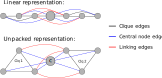
\includegraphics[width=0.7\textwidth]{lcp.pdf}
    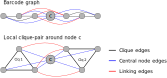
\includegraphics[width=0.7\textwidth]{lcp_2.pdf} %RC: minor cosmetic changes
    \caption{(Top) linear representation of a barcode graph obtained from $7$ molecules of uniform length. (Bottom) The local clique-pair associated to $c$. In black, the edges from the side cliques of the unit 3-graph. In blue, the edges between the central nodes and the other nodes. In red, the edges between the cliques.}
    \label{fig:perfect_udg}
\end{figure}

To motivate the introduction of lcps, we ran an experiment described in Appendix~\ref{appendix:perfectlcps}, that shows that the rate of lcps that actually encode the barcodes of consecutive molecules is higher than the rate of maximal cliques having the same property (Table~\ref{tab:clqvslcp}).
%Table~\ref{tab:clqvslcp} shows that the proportion of perfect lcps (13.5-50\%) is higher than the proportion of maximal cliques (8-9\%) in synthetic barcode graphs, motivating the use of lcps instead of maximal cliques for realizing barcode graphs.

We now discuss our algorithm to compute lcps.
Given a barcode $c$, there can be many maximal cliques among nodes in its neighborhood, especially cliques that involve the two barcodes that respectively precede and follow $c$ in the true barcode sequence.
%We do not want to keep those cliques within a lcp centered at $c$.\footnote{RC to YD: I don't understand why we don't want these cliques. Can you elaborate why? YD: I don't remind me writing that. Maybe a remnant part from older versions. I delete}
Given the set of all maximal cliques, we thus need to extract a matching defining pairs of cliques $C_1$ and $C_2$ forming lcps.
To do so, given the set of all maximal cliques in the neighborhood of $c$, we consider the complete graph whose vertices are maximal cliques and edges are putative lcps.
Let $W$ be the maximum observed lcp weight among these potential lcps. 
We replace the weight $w$ of each lcp by $W-w$ and apply a maximum-weight matching to 
clique pairs in order to obtain the set of lcps associated to $c$ (Algorithm~\ref{algo:audg}, illustrated in Fig.~\ref{fig:mwm}).

\begin{algorithm}
    \caption{Determination of a set of lcps centered at a barcode $c$.}
    \label{algo:audg}
    \begin{algorithmic}[1] % The number tells where the line numbering should start
        \Procedure{compute\_Lcp}{$c, BG$} \Comment{c: barcode, BG: barcode graph}
            \State $LCP \gets$ \O
            \State $nbs\gets BG.neighbors(n)$
            \State $subgraph \gets BG.induced\_subgraph(nbs)$
            \State $cliques \gets subgraph.max\_cliques()$ \Comment{Enumerate maximal cliques}
            \State $CG \gets clique\_graph(cliques)$ \Comment{Clique graph from divergences}
            \State $m = CG.maximum\_weight\_matching()$
            \For{$(C_1, C_2) \in m$}
                \State $LCP \gets LCP \cup new\_lcp(c, C_1, C_2)$ \Comment{Add the new Lcp}
            \EndFor
            \State \textbf{return} $LCP$
        \EndProcedure
    \end{algorithmic}
\end{algorithm}
%\footnote{Rayan to Yoann: what are $U$ and $Lcp(x,y,z)$ in the algorithm?\\
%Y: $U$ a typo from a previous version, $LCP$ the set of all generated LCP centered on $x$.}

\begin{figure}[htp]
    \centering
    %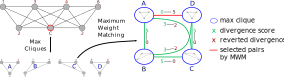
\includegraphics[width=\textwidth]{mwm.pdf}
    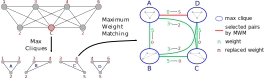
\includegraphics[width=.95\textwidth]{mwm_v2.pdf} % RC: made some cosmetic changes
    \caption{Top left: barcode graph; bottom left: max-cliques of the barcode graph; right: max-clique graph construction and maximum weight matching to construct lcps.}
    \label{fig:mwm}
\end{figure}

The time complexity of enumerating all maximal cliques of a graph is exponential~\cite{TomitaTT_2006}, while computing a maximum-weight matching is polynomial-time solvable~\cite{Galil_1986}. 
We implemented Algorithm~\ref{algo:audg} in Python using the output-sensitive cliques enumeration and maximum-weight matching methods implemented in the Networkx library~\cite{HagbergSS_2008}. Its complexity is $O(\max(C^3, M(n) C))$ with $n$ the number of graph nodes, $C$ the number of maximal cliques in the graph, and  $M(n)$ the cost of multiplying two $n\times n$ matrices.
%\footnote{CC. Est-ce qu'on peut \^etre plus or\'ecis sur le temps d'ex\'ecution?\\
% RC: oui surement.. Yoann, tu tilises \texttt{find\_cliques()} de networkx?
 %si oui, le papier cité % %https://www.sciencedirect.com/science/article/pii/S0304397508003903?via%3Dihub
 %par networkx dit: " all maximal cliques of a n vertices graph can be enumerated using $n^2$ %space, and with time delay $O(M(n))$ with $M(n)$ the cost of multiplying two n × n %matrices."\\
 %Y: D'accord avec Rayan sur le find\_cliques, puis $n^3$ pour le matching, n étant le nb de %maxcliques sorties par l'étape précédente.}
%\todo[inline]{CC. je ne suis pas s\^ur de comprendre la figure. Surtout les cliques sont disjointes, ce qui est contre-intuitif je pense. Si on cherche toutes les cliques maximales dans un voisinage on ve surement en avoir qui partage un (ou plusieurs) sommet(s).}
%\todo[inline]{Figure 2 will change according to CC's comment: Si on prend un exemple simple, 3 molecules avant c (1,2,3) et 3 molecules apres (4,5,6) espac\'ees r\'eguli\`erement, on a 4 cliques maximales, (1,2,3,c), (2,3,4,c), (3,4,5,c), (4,5,6,c) et le MWM ressort deux lcps, (c,(1,2,3),(4,5,6)) et (c,(2,3,4),(3,4,5)) et on est pass\'e de 4 cliques maximales \`a deux lcps. Mais il est difficile de discuter de la qualit\'e d'un tel r\'esultat sans parler de comment on utilise ces lcps par la suite.}

Local search for linked cliques are akin to local graph community detection.
Soft clustering is being performed with maximal clique detection, i.e. a node may belong to multiple communities.
This property leads to a lcp detection algorithm that, intuitively, is resilient to the situation where a barcode corresponds to strictly more than 2 molecules. Yet our algorithm is not perfect: it can also generate lcps that do not reflect a collection of overlapping molecules (due to additional artifactual maximal cliques); and also, missing edges in the barcode graph may lead to missing lcps.

In the ideal case, lcps can be totally ordered according to their overlaps. But because of artefactual and missing lcps, a total order is not always self-evident.
By introducing the concept of lcp graph, we are creating a new structure that can reveal a large linear lcp successions and filter out lcps that are not overlapping with others.

\begin{definition}
    \label{def:lcp_graph}
    Let $BG$ be a barcode graph and $V$ a set of lcps obtained from $BG$. The lcp graph $lcp(BG)$ is the weighted graph with $V$ for vertex set and where there is an edge between two lcps $(b;B_1,B_2)$ and $(c;C_1,C_2)$ such that some barcode belongs to both one of the $C_i$ cliques and one of the $B_i$ cliques. The weight of an edge is the size of the symmetric differences of the barcodes content of $(b;B_1,B_2)$ and $(c;C_1,C_2)$. 
\end{definition}

The figure \ref{fig:deconv} highlight the linear structures revealed by the lcp graph on synthetic barcodes.

In the following, we will describe how we determine a barcode ordering based on finding a path in the lcp graph.

%\todo[inline]{CC. Mon commentaire est plut\^ot que la remarque utilise un vocabulaire impr\'ecis (resilient, multiple local merges, wrong udg, missing udg) ce quei la rend difficile \`a comprendre. C'est plus une question de reformulation, mais qui rejoint mon commentaire plus haut sur la difficult\'e d'interpr\'eter les udg/lcp en isolation d'un algorithme qui traverse le graphe.
%RC: d'accord avec la remarque de CC, qui pourrait être adressée en étant plus précis sur le 'multiple local merges' et 'wrong and others are missing': par exemple en donnant un exemple d'udg incorrect (et d'un manquant, mais je réalise que pour manquant c'est peut-être pas facile de construire un tel exemple).}


% Rayan to Cedric:  j'ai enlevé cette partie, suite à une discussion avec Yoann, qui pense que ce n'est pas toujours vrai pour 2 raisons:
% - aux bords du barcode graphe, le lcp risque de ne pas trouver le bon ordre des barcodes car il n'y aura pas de cliques
% - si basses couvertures, alors on pourrait avoir des d-graphes avec d=1 et du coup, pas vraiment de possibilité de trouver de lcp
% donc il faudrait surement définir précisément des conditions 'idéales' plus précises pour avoir le résultat que tu escomptes
%\todo[inline]{CC. Je pense que le bout de texte suivant est vrai. Ca pourrait valoir le coup de le prouver.}
%It is straightforward\todo{CC. A prouver \dots peut-\^etre difficile \`a cause des intervalles-extr\'emit\'es qui n'ont pas de lcp.}  to see that, in the case where each barcode labels exactly one molecule and $BG$ is an exact barcode graph, then $BG$ is an interval graph and one can obtain easily from the lcp graph a realisation of $BG$ which is the true barcode sequence. While this is not an optimal way to realise an interval graph due to the maximal cliques computation, this shows that the concept of lcp graph is relevant for the problem of molecules ordering.

%\todo[inline]{CC. Ma d\'efinition du poids d'une ar\^ete est peut-\^etre fausse. Elle correspond \`a mon interpr\'etation de sommet extr\^eme, mais je ne suis pas s\^ur d'avoir compris.} % Yoann a dit que c'est OK

%\todo[inline]{CC. Pr\'esent\'e comme cela, sans exemples, j'ai peur qu'un arbitre puisse penser qu'on a cr\'e\'e une structure qui est en fait plus lourde que le barcode graph et difficile \`a analyser. Il faut soit des exemples visuels qui montrent que ce graph est plus lin\`eaire qu'un barcode graph, soit un algorithme de layout avec des r\'esultats.}


% ancien texte a cette section:
%TODO: Voir avec Rayan pour utilisation threshold/moyen plus malin.
%Interesting assembly properties.
%Cedric work on path retrieving ?\todo{Non car je n'ai pas de r\'esultats \`a montrer.}
%conclusion: More interesting solution for counting problem (filter out a lot of wrong udgs).
%Assembly process allow to traverse the graph and try to extract total order.

\begin{figure}
\includegraphics[height=4cm]{figs/simu_0_bar_n10000_d10_m3-dev1.gexf.png}\hspace{1cm}
\includegraphics[height=4cm]{figs/simu_0_bar_n10000_d10_m3-dev1_d2_simplified_maxclq-cropped.pdf}\hspace{1cm}
    \centering
    %\includegraphics{}
    \caption{Left: barcode graph of a simulated interval graph, 3k nodes and 98k edges. Right: Resulting lcp graph, 13k nodes and 23k edges. (Gephi, ForceAtlas 2 layout~\cite{gephi})}
    \label{fig:deconv}
\end{figure}


\subsection{Finding a suitable path in the lcp graph \label{sec:suitable_path}}

Recall that the molecule counting problem amounts to finding how many molecules were merged in each barcode. The molecule ordering problem asks for a sequence of barcodes that reflecst the order of molecules. As these two problems are centered on barcodes, we need a way to convert a lcp path into an ordered list of barcodes.  We do this as follws: each lcp in the path is replaced by its central barcode. %This simplification is a good proxy to approximate the barcode succession instead of the lcp succession.

Figure \ref{fig:deconv} illustrates that the lcp graph constructed from a synthetic barcode graph has a visibly linear structure. This makes the task of finding a suitable path within the lcp graph that reflects the ordering of molecules easier than in the barcode graph. 
To do this, we perform two steps: i) edge reduction within the lcp graph to remove redundant edges, and ii) a greedy algorithm with local branch and bound refinements which finds an initial path and improves it.

\paragraph*{lcp graph simplification} We simplify the lcp graph by performing transitive reduction over triplets.
Given an edge $(a,b)$ of weight $w_{ab}$, we remove this edge from the graph if there exist 2 edges $(a,c)$ of weight $w_{ac}$ and $(b,c)$ of weight $w_{bc}$ such that $w_{ab} \leqslant w_{ac} + w_{bc}$.
This operation does not change the node set (lcps) but reduces the number of possible paths to explore.
Intuitively, requiring to go through lcp $c$ when going from lcp $a$ to lcp $b$ forces to select two higher-confidence lcp overlaps instead of one lower-confidence lcp overlap.

\paragraph*{lcp path construction}

Assuming the barcode graph has been obtained by merging nodes of the exact interval graph defined by the molecules intersections, every edge of the barcode graph does correspond to one (or potentially several) edges of this interval graph; we show in Section~\ref{sec:bg_reads} that barcode graphs created from reads have nearly all correct edges corresponding to such molecules intersections.
%Toward solving the problem of computing a walk in the lcp graph that reflects the true order of molecules, this observation motivates to require that such a walk should be composed of lcps that contain most of the edges of the original barcode graph.
This observation motivates to require that a walk in the lcp graph that reflects the true order of molecules should be composed of lcps that contain most of the edges of the original barcode graph.
We define a \textit{covering variable} $v_i$ for each edge $e_i$ of the barcode graph.
Each lcp is an induced subgraph of the barcode graph, so it can be associated to a set of covering variables, i.e. edges of the barcode graph.
We will seek a path such that the union of covering variables over all its constituent lcps is as close as possible to the set of all covering variables.%\footnote{RC to YD: better?}

Our lcp path construction strategy is a local branch \& bound algorithm.
Assuming we have already constructed a path of lcps $p = l_1,\ldots,l_i$, we consider as candidates for $l_{i+1}$ all the neighbors of $l_i$ in the lcp graph such that $l_{i+1}  \notin p$.
Those neighbors are sorted by priority over three criteria: first if one or more lcp(s) cover at least one uncovered variable, i.e. one edge of the original barcode graph, we restrict our choice to those lcps. \footnote{RC to YD: it seems that this first criterion isn't about sorting but rather removal of some candidate lcps. Is that true or did I make a mistake when rewriting that part? YD: They are not completely removed. We try first the paths with the node that come first in the sorted neighbors but the other nodes can be bridges so we try them if nothing else worked} % (otherwise, we choose the extension among all neighbors of $l_i$.
For the second sorting criterion,  we sort the candidate $l_{i+1}$'s by increasing clique pair weight. %\footnote{RC to YD: you mean lcp graph weight? YD:    No, lcp divergence. It has been recently renamed the weight of the clique pair}.
Last, if multiple candidates have equal clique pair weights, we sort them by increasing $l_i \rightarrow l_{i+1}$ edge weight in the lcp graph.
Selecting the first element in the sorted neighbors at each step defines a greedy heuristic for the path computation.

The above algorithm might result in a short path due to tips in the lcp graph, i.e. nodes of degree $1$.
In order to address this issue, we use a local branch and bound algorithm and backtrack a few nodes when a dead end is reached.
This can result in several paths and we use the number of covering variables in the path as a score to keep only the best solutions according to that score.

The last part of the algorithm is the selection of the first node $l_1$ of the path.
Because we do not have good selection criteria, we initially select a $l_1$ at random among all lcps.
We start by computing a path using the above algorithm which ends at some node $l_e$.
We then discard this part and restart again our algorithm from $l'_1 = l_e$ to create a new path, where $l_e$ has a higher chance to be an endpoint of the true lcp path than $l_1$.

%\todo[inline]{CC: I do not understand as from my understanding of the part above, $n_e$ is a dead-end.\\
%YD: Yes but we hope that it's the farthest reachable node.
%RC: I reformulated that part. }

We will show in the next section that despite this heuristic being very simple and likely leaving  room for improvement, it does work very well on simulated data, suggesting the lcp graph does actually capture a very robust signal toward recovering the correct barcode sequence.

%Of course, this heuristic is not perfect and will not always find a perfect solution. But it is sufficient to prove that retrieving a good path from our lcp graph is feasible, even with naive algorithms.


%\paragraph*{Counting molecules in path}

%%%%%%%%%%%%%%%%%%%%%%%%%%%%%%%%%%%%%%%%%%%%%%%%%%%%%%%%%%%%%%%%%%%%%%%%%%%


%%%%%%%%%%%%%%%%%%%%%%%%%%%%%%%%%%%%%%%%%%%%%%%%%%%%%%%%%%%%%%%%%%%%%%%%%%%

\section{Results}

Our results consider various types of simulated data. We described below how we generate these data and our analysis, before dicsussing our results.

\subsection{Simulations set-up}

\subsubsection*{Simulated data}

We will examine three types of barcode graphs ordered by increasing level of realism. They will be generated from either
\begin{enumerate}
\item entirely synthetic sets of intervals (i.e. interval graphs) with randomly identified vertices,
\item intersections of molecules sampled from a genome, 
\item directly from simulated linked-read sequencing data.
\end{enumerate}
%The purpose of this section is to evaluate the quality of lcp graphs generated by our method and their ability to recover the underlying molecule order, as well as perform molecule counting.

\subsubsection*{Analysis pipeline}

%Recall that the molecule counting problem amounts to finding how many molecules were merged in each barcode. The molecule ordering problem asks for a sequence of barcodes that reflecst the order of molecules.
%
%As these two problems are centered on barcodes, we need a way to convert a lcp path to an ordered list of barcodes. \footnote{RC: I'm thinking of moving that part to the Methods are going from lcp path to central nodes is a choice we make towards constructing the sequence of barcodes. CC: I agree, this should be in the methods section.} For the results we will use the following simplification: each lcp in the path is replaced by its central barcode.
%This simplification is a good proxy to approximate the barcode succession instead of the lcp succession.

Our complete analysis pipeline performs the following steps:
\begin{enumerate}
    \item Generate all the lcps from the barcode graph (Algorithm~\ref{algo:audg})
    \item Generate the lcp graph
    \item Simplify the graph by transitive reduction of the triplets (Section~\ref{sec:suitable_path})
    \item Generate the lcp path using the hybrid greedy/branch and bound algorithm (Section~\ref{sec:suitable_path})
    \item Replace all the lcp by their central barcodes
    \item Evaluate the accuracy of the resulting barcode sequence
\end{enumerate}

In the remaining of the Results sections, all the graphs and paths are generated by the above  pipeline, implemented using \texttt{Snakemake} and available at \url{https://gitlab.pasteur.fr/ydufresne/linkedreadsmoleculeordering}.

\subsubsection*{Quality metrics}

We want to analyze the quality of the lcp graph regarding the barcode graph from which it was computed.
To be comparable, we transformed the nodes of the lcp graphs by replacing the lcps by their central barcode.
We consider three metrics over the graphs: accuracy, sensitivity and longest increasing path. The first two metrics are estimated by randomly sampling paths having $l=2,4,10,100$ edges from the graph. To measure accuracy, a path having central nodes $(p_0,p_2,\ldots,p_l)$ is considered to be correct if there exists $m_0,m_2,\ldots,m_l$ overlapping (but not necessarily consecutive) molecules such that $m_i \in m(p_i)$, $0\leq i\leq l$. Accuracy is then defined as the number of correct paths over the total number of sampled paths. 
To measure sensitivity, we determined for all $(l+1)$-tuples $m_i,m_{i+1},\ldots,m_{i+l}$ of consecutive molecules in the genome, whether there exist a path $b(m_i),b(m_{i+1}),\ldots,b(m_{i+l})$ in the graph. Sensitivity is then the ratio of such paths that are found in the graph.   
Finally, the Longest Correct path (LC) metric is defined as the longest path that can be found in the lcp graph that is correct, i.e. corresponds to a barcode sequence equal to the barcodes of a sequence of overlapping molecules. This measure is not informative over the barcode graph, because it is conservative regarding the molecule path. It measure the conservation of information when the lcp graph is created.
  
Two additional quality metrics are defined on lcp paths: Undercounted/Overcounted (U/O) molecules and Longest Common Subsequence (LCS).
The U/O metric is computed by recording two counters, $U$ and $O$ initialized at 0. Given each barcode $b$ that appears within a lcp path, we compare the number of occurrences of $b$ to $M_b$, the true number of molecules having barcode $b$. If $b$ occurs in the lcp path strictly more (resp. less) than $M_b$ times, $U$ (resp. $O$) is incremented by the absolute difference. U and O should both be as close to zero as possible, and they indicate how well we solve the molecule counting problem. 
For the LCS metric, we compute the longest common subsequence between central nodes of the lcp path and the molecule path where each molecule is replaced by its barcode. The LCS reflects how well we solve the molecule ordering problem.

%\todo[inline]{CC: We need to discuss the link between LIS and LCS. RC: LIP you mean? We don't really talk about longest increasing subsequence in the article. I renamed LIP to LC}

\subsection{Simulated data from interval graphs}

\subsubsection*{Dataset generation}

At first we focus on purely synthetic interval graphs, where a genome is conceptually a real line and molecules are intervals on this line.
We make the simplifying assumption that molecules all have the same size, and are evenly distributed along the genome.
%As described in the section \ref{sec:interval_graph}, we transform this representation into an interval graph.
%We then remove random nodes from this ideal graph to simulate local variations on molecule overlap.\footnote{RC to YD: do we do that?! if so, how many? I thought that Table 1 had exactly 5000 (and 10000) molecules, not 5000 minus some randomly deleted ones. YD: You are right. It is an experiment from the past}
%The resulting graph is our ground truth for the next parts.

To simulate barcode graphs, we start from an intersection graph of molecules and perform so-called \emph{merges} of molecules. A merge is defined as follows: given two nodes $a$ and $b$ that will be merged, create a new node $c$; for all neighbors $v$ of either $a$ or $b$, create edges $(c,v)$, and finally delete $a$ and $b$.
Merging two nodes in the graph is equivalent to replacing two molecules by one barcode corresponding to those two molecules. A succession of merge operation creates an exact barcode graph as defined in Section~\ref{sec:methods}. %i.e. the merges do not create false edges.

%The average number of merges is the average molecule nodes that have been merged into a single node of the BG, and the merge deviation as its standard deviation.
%These two values are used to generate variations on experiment parameters in the next sections.
% RC: removed as we don't use these terms later

We created 8 synthetic test datasets, using the following grid of parameters: $5,000$ or  $10,000$ molecules, average number of merges (i.e. molecules per barcode) of $2$ or $3$, standard deviation in the number of merges of 0 or 1. %Inside of our simulated barcode graph we keep track of the molecule merged (ordered from 1 to length).

\subsubsection*{Analysis}

Table \ref{tab:simu_accsens} shows the accuracy and sensitivity of barcode graphs and their corresponding lcp graphs.
% As expected, the accuracy mesure show that the barcode graph is not well ordered.
Recall that accuracy measures whether a random path in the graph has a correct order of barcodes. As expected, paths in the barcode graph are mostly inaccurate, as one may jump from one genome location to another due to barcode merges. Conversely paths in the lcp graph are very accurate ($100\%$ for nearly all $l=10$ paths), with a slight decrease at $l=100$ ($95\%-100\%$). The sensitivity metric measures how much of the true barcode ordering is present in short paths of the graph. It is naturally high for barcode graphs, as they preserve all overlaps between molecules.
Note that some merges collapse consecutive molecules by chance, hence the sensitivity of barcode graphs is not always 1. On lcp graphs, sensitivity is high for short paths ($>93\%$ for $l=10$) and drops for long ones ($54\%-98\%$ for $l=100$).
Nevertheless, this shows that at least partial molecule order can indeed be inferred by only looking at central nodes of lcps in the lcp graph, and that the lcp graph shows a better balance between accuracy and sensitivity than the barcode graph. Note that this is not the only way to infer molecule order, as one could also extract information from clique-pairs, yet we leave this direction for future work.

Overall, lcp graphs are clearly more informative than barcode graphs for reconstructing accurate barcode orderings. The hardest instances, in terms of accuracy and sensitivity on lcp graphs, are when the number of molecules is low and the number of merges is high. 

\begin{table}

\begin{tabular}{|p{1cm}|p{1cm}|p{.7cm}||p{1cm}|p{1cm}|p{1cm}|p{1cm}|p{1cm}|p{1cm}|p{1cm}|p{1cm}|  }
 \hline
   % &\multicolumn{2}{c|}{\textbf{l=1}} % not so interesting, everything is correct for those values
   \multicolumn{3}{|c||}{\textbf{Graph}}
   & \multicolumn{2}{c|}{\textbf{l=2}}
   %& \multicolumn{2}{c|}{\textbf{l=3}}
   & \multicolumn{2}{c|}{\textbf{l=4}} 
   & \multicolumn{2}{c|}{\textbf{l=10}}
   & \multicolumn{2}{c|}{\textbf{l=100}} 
   \\
 \hline
\# mols & Merges & Type  & Acc & Sens & Acc & Sens & Acc & Sens & Acc & Sens \\

    \hline
    \hline
    \multirow{2}{*}{5,000} & \multirow{2}{*}{2 $\pm$ 0} & $G_b$ & 0.48 & 1.00 & 0.09 & 1.00 & 0.00 & 0.99 & 0.00 & 0.94\\
     & & lcp & 1.00 & 1.00 & 1.00  & 0.99 & 1.00 & 0.98 & 1.00 & 0.88 \\
    \hline
    \multirow{2}{*}{5,000} & \multirow{2}{*}{2 $\pm$ 1} & $G_b$ & 0.46 & 1.00 & 0.09 & 1.00 & 0.00 & 1.00 & 0.00 & 0.98\\
    & & lcp & 1.00 & 1.00 & 1.00 & 0.99 & 1.00 & 0.98 & 0.99 & 0.84 \\
    \hline
    \multirow{2}{*}{5,000} & \multirow{2}{*}{3 $\pm$ 0} & $G_b$ & 0.31 & 1.00 & 0.03 & 1.00 & 0.00 & 0.99 & 0.00 & 0.88\\
    & &  lcp& 1.00&  0.99 & 1.00 & 0.98 & 0.99 & 0.95 & 0.99 & 0.60 \\
    \hline
    \multirow{2}{*}{5,000} & \multirow{2}{*}{3 $\pm$ 1} & $G_b$ & 0.33 & 1.00 & 0.03 & 1.00 & 0.00 & 1.00 & 0.00&  0.96\\
    & & lcp & 1.00 & 0.99 & 1.00 & 0.97 & 0.99 & 0.93 & 0.95 & 0.54 \\
    \hline
    \multirow{2}{*}{10,000} & \multirow{2}{*}{2 $\pm$ 0} & $G_b$ & 0.48 & 1.00 & 0.10 & 1.00 & 0.00 & 1.00 & 0.00 & 1.00\\
    & & lcp & 1.00 & 1.00 & 1.00 & 1.00 & 1.00 & 1.00 & 1.00 & 0.98 \\
    \hline
    \multirow{2}{*}{10,000} & \multirow{2}{*}{2 $\pm$ 1} & $G_b$ & 0.47 & 1.00 & 0.09 & 1.00 & 0.00 & 1.00 & 0.00  & 0.97\\
    & & lcp & 1.00 & 1.00 & 1.00 & 1.00 & 1.00 & 0.99 & 0.99 &  0.93 \\
    \hline
    \multirow{2}{*}{10,000} & \multirow{2}{*}{3 $\pm$ 0} & $G_b$ & 0.31&  1.00 & 0.02 & 1.00 & 0.00 & 1.00 & 0.00  &1.00\\
    & & lcp & 1.00 & 1.00 & 1.00 & 0.99 & 1.00 & 0.99 & 1.00 & 0.87\\
    \hline
    \multirow{2}{*}{10,000} & \multirow{2}{*}{3 $\pm$ 1} & $G_b$  &0.31 & 1.00 & 0.03 & 1.00 & 0.00 & 1.00 & 0.00  &0.97\\
    & & lcp & 1.00 & 0.99 & 1.00 & 0.99 & 1.00 & 0.97 & 0.99  & 0.78\\
    \hline
 \end{tabular}
\caption{Same as Table 2 but for interval graphs. Let's see how we present this.\label{tab:simu_accsens}}
\end{table}

Table \ref{tab:synthetic_results} reports additional barcode graphs metrics over the same 8 datasets.
All barcode graphs have a high longest correct path (LC), confirming the theoretical possibility of reconstructing over 99\% of the true barcode order, through central nodes of a suitable path of lcps.
The last two metrics of Table \ref{tab:synthetic_results} are computed on lcp paths found by the algorithm described in Section~\ref{sec:suitable_path}. On 10,000 molecules graphs, the longest common subsequence (LCS) of the computed lcp path is 90\% of the true barcode order, indicating that we nearly recovered the correct barcode order. The 5,000 molecules graphs appear to be more challenging to process as, smaller graphs are more sensitive to information loss by the merging process, yet LCS remain above $79\%$. %But we think that smarter algorithms can reconstruct the path because of the size of the LC.
The U/O metric reports the ability to count the number of molecules that are present in each barcode, though counting the number of times each barcode occurs in the computed lcp path. %Almost all the barcodes that correspond to well placed lcps in the path lead to a correct barcode counts and missing lcps lead to undercounts.
Overall, lcp paths tend to undercount molecules (higher $U$ metric than $O$), yet both $U$ and $O$ metrics are around or below $10\%$ of the number of molecules, indicating that lcp path provides a reliable estimation of the number of molecules per barcode.

%To conclude on the values from the table \ref{tab:synthetic_results}, the lcp graph appears to be a good structure to extract paths from it.
%Even simple path construction heuristics can extract a good approximation of molecule counts and barcode orderings.

\begin{table}
\begin{tabular}{|l|l|l||l|l|l||l|l|}
    \hline
    \# mols & Merges & \# barcodes & LC & U/O Counts & LCS \tabularnewline
    \hline
    \hline
    5,000 & 2 $\pm$ 0 & 2500 & 4990 & 227/56 & 4748  \tabularnewline
    \hline
    5,000 & 2 $\pm$ 1 & 2428 & 4991 & 405/109 & 4512  \tabularnewline
    \hline
    5,000 & 3 $\pm$ 0 & 1667 & 4985 & 549/240 & 4282 \tabularnewline
    \hline
    5,000 & 3 $\pm$ 1 & 1682 & 4975 & 498/665 & 3972 \tabularnewline
    \hline
    10,000 & 2 $\pm$ 0 & 5000 & 9992 & 268/68 & 9667  \tabularnewline
    \hline
    10,000 & 2 $\pm$ 1 & 4889 & 9993 & 418/129 & 9531  \tabularnewline
    \hline
    10,000 & 3 $\pm$ 0 & 3334 & 9981 & 593/184 & 9309  \tabularnewline
    \hline
    10,000 & 3 $\pm$ 1 & 3341 & 9987 & 753/201 & 9140  \tabularnewline
    \hline
 \end{tabular}
\caption{Experiments on synthetic barcode graphs. The dataset is described on the first part of the columns (Number of molecules in the molecule graph, merging factors, resulting number of barcodes in the barcode graph). The LC column is the length of the longest correct path in the lcp graph. The U/C column is the number of undercounted and overcounted molecules per barcode in our computed lcp path, and the LCS column is the length of the longest common subsequence between the lcp path and the correct barcode order.
\label{tab:synthetic_results}}
\end{table}

\subsection{Genome graphs}

\subsubsection*{Quality of genome LCP graphs}


\begin{table}
\begin{tabular}{ |p{2.3cm}||p{1cm}|p{1cm}|p{1cm}|p{1cm}|p{1cm}|p{1cm}|p{1cm}|p{1cm}|  }
 \hline
   % &\multicolumn{2}{c|}{\textbf{l=1}} % not so interesting, everything is correct for those values
   & \multicolumn{2}{c|}{\textbf{l=2}}
   %& \multicolumn{2}{c|}{\textbf{l=3}}
   & \multicolumn{2}{c|}{\textbf{l=4}} 
   & \multicolumn{2}{c|}{\textbf{l=10}}
   & \multicolumn{2}{c|}{\textbf{l=100}} 
   \\
 \hline
\textbf{Graph}  & Acc & Sens & Acc & Sens & Acc & Sens & Acc & Sens \\
\hline
\hline
\textbf{$G_b$, $m=1$} &
 %1 &1 & % l = 1
 1 & 1 & % l = 2
 % 1&1 & % l = 3
 1 & 1 & % l = 4
 1 & 1 &  % l = 10
 1 & 1 % l = 100
 \\
 \textbf{$lcp$, $m=1$} &
 %1 & 1  &  % l = 1
 1 & 1 &  % l = 2
 %1 & 1 & % l = 3
 1 & 0.99 & % l = 4
 1 & 0.99 &  % l = 10
 1 & 0.84  % l = 100
 \\
 \hline
 \textbf{$G_b$, $m=2$} & 
 %1 & 1  &  % l = 1
 0.50 & 1 &  % l = 2
 %0.25 & 1 & % l = 3
 0.12 & 0.99 & % l = 4
 0.001 & 0.99 &  % l = 10
 0 & 0.99     % l = 100
 \\
 \textbf{$lcp$, $m=2$} &
 %1 &1  &  % l = 1
 0.99 & 0.99 &  % l = 2
 %0.99 & 0.99 & % l = 3
 0.99 & 0.99 & % l = 4
 0.99 & 0.99 &  % l = 10
 0.94 & 0.84   % l = 100
 \\
 \hline
 \textbf{$G_b$, $m=3$} & 
 %1 & 1 & % l = 1
 0.34 & 1 &  % l = 2
 %0.12 & 1 & % l = 3
 0.04 & 1 & % l = 4
 0 &  1   &  % l = 10
 0 &  1      % l = 100
 \\
 \textbf{$lcp$, $m=3$} &
 %1 &1 &  % l = 1
 0.99 & 0.99 &   % l = 2
 %0.99 & 0.99 & % l = 3
 0.99 & 0.99 & % l = 4
 0.98 & 0.99 &  % l = 10
 0.88 & 0.88 % l = 100
 \\
 \hline
 \textbf{$G_b$, $m=4$} & 
 %1 & 1 &  % l = 1
 0.26 & 1 &  % l = 2
 %0.07 & 1 &  l = 3
 0.02 & 0.99 & % l = 4
 0 & 0.99 & % l = 10
 0 &  0.99  % l = 100
 \\
 \textbf{$lcp$, $m=4$} &
 %1 &1 & % l = 1
 0.99 & 0.99  &  % l = 2
 %&  & % l = 3
 0.99 & 0.99 & % l = 4
 0.98 & 0.99 &  % l = 10
 0.83  & 0.87  % l = 100
 \\
 \hline
\end{tabular}
\caption{Accuracy and sensitivity of randomly sampled paths of lengths 2, 4, 10 and 100 edges in lcp graphs, compared to sampled paths of the same lengths in barcode graphs ($G_b$) as a base-line, with 15 kbp E. coli molecules, 50X coverage, minimal molecule overlap lengths of 7000. \label{tab:d2-local-quality}}
\end{table}

We designed experiments to evaluate the quality of lcp graphs constructed from the barcode graphs that originate from real molecules. We created a synthetic \emph{E.coli} molecule graph by simulating molecules of length 15 kbp using \texttt{wgsim}, corresponding to sequences of the E. coli genome, at 50x coverage of the genome and with no sequencing errors. Overlaps between all pairs of molecules were computed using \texttt{minimap2} using default parameters, and we selected only overlaps of lengths $L$ ($L=6000,7000,8000,9000$) using \texttt{fpa}~\cite{fpa}. 



%We randomly merged $k$ molecules ($k=2,3,4,5$) to create synthetic barcode graphs of these molecules. We constructed lcp-graphs from these barcode graphs.

%We then evaluated the quality of the lcp-graphs by computing  two metrics: accuracy and sensitivity. These metrics were obtained by randomly samplings paths having $l=2,4,10,100$ edges from the lcp-graphs. Each sampled path is converted into a succession of barcodes by taking the central node of each lcp node.  To measure accuracy, a path having central nodes $(p_1,p_2,\ldots,p_l)$ is considered to be correct if there exists a succession $m_0,m_2,\ldots,m_{l+1}$ of overlapping molecules (e.g. a path from the original molecule graph) such that $m_0 \in m(p_0), m_2 \in m(p_2)$, \ldots, $m_l \in m(p_l)$. Accuracy is defined as the number of correct paths over the total number of sampled paths. 
%To measure sensitivity, we determined for all $(l+1)$-tuples $m_i,m_{i+1},\ldots,m_{i+l}$ of consecutive molecules, whether there exist a path of central nodes $b(m_i),b(m_{i+1}),\ldots,b(m_{i+l})$ in the lcp-graph graph. Sensitivity is then the ratio of such paths that are found in the lcp-graph.  

Table~\ref{tab:d2-local-quality} shows the accuracy and sensitivity on our constructed lcp graphs versus the average number of merges, i.e. average number of molecules per barcode. Barcode graphs have poor accuracy, which is expected due to the glueing of molecules, but perfect sensitivity as all molecule overlaps are found. In contrast, lcp-graphs manage to keep both near-perfect accuracy and sensitivity ($>0.98$) for short paths ($<10$) and have a decrease in accuracy ($0.83-0.94$) and sensitivity $(0.84-0.87)$ for paths of length $100$.


\subsubsection*{Construction of genome barcode graphs from reads \label{sec:bg_reads}}

In this section we describe a method that constructs an accurate barcode graph directly from linked-read data. This closes a gap between our theoretical results, that required to already have a barcode graph, and experimental data which only consist of sequencing reads.

We simulated reads from the \emph{E. coli} genome at 50X coverage using LRSIM. We assembled these reads using SPAdes version 3.12.0 without using linked-read information (only using paired-end information), in order to generate contigs to which linked-reads can be mapped to using the EMA aligner. We designed an algorithm to infer molecule overlaps given the set of contigs and the EMA alignments. In brief, the algorithm proceeds as follows

For each barcode, and all reads associated that barcodes mapped to a contig, we collect and sort read mapping positions. We define a molecule interval to be the first and last mapping positions of a group of mapping positions that are all within a distance $<$ $M_d$ than each other. A barcode can be associated to many molecule intervals even within the same contig. We construct the barcode graph by looking at overlapping molecule intervals from different barcodes. If two intervals share an overlap larger than a parameter $M_o$, we add an edge between the two associated barcodes.


\begin{figure}
    \centering
    \includegraphics[width=.68\textwidth]{barcode_graph_optimisation.pdf}
    \caption{Quality of barcode graph construction from a set of reads and corresponding paired-end assembly. Each square represents the F1-score given parameters $M_d$ (read mapping distance) and $M_o$ (minimal molecule overlap length), from  purple (low F1-score) to yellow (high F1-score). %The lowest F1-score is 0.032 for $(M_d M_o) = (10000, 1000)$, the highest (square in red) is 0.953 for $(M_d, M_o) = (9000, 5000)$
    }
    \label{fig:barcode_graph:parameter_opti}
\end{figure}


The algorithm has two key parameters: $M_d$, the maximal distance between two reads in an inferred molecule interval, and $M_o$, the minimal overlap length between molecules. As we used simulated data, we were able to generate a ground-truth barcode graph given that molecule intervals in the underlying genome are known for each barcode. Figure \ref{fig:barcode_graph:parameter_opti} shows the performance of the algorithm in terms of F1-score (combining both sensitivity and precision, computed by comparing the edge set of the inferred barcode graph versus the edge set of the ground truth). We observe that the best F1-score (0.953) is reached for $(M_o, M_d) = (5000, 9000)$, with otherwise consistently high F1-scores ($\geq0.9$) whenever $M_o>2000$ and $M_d>7000$.

%\subsection{If we have time: molecule counting vs Minerva}

%$ python ~/10x-deconvolve/deconvolution/main/minerva_molecule_counting.py
%minerva reported 2003 barcodes 5977 molecules
%original reads contained 2938 barcodes 11926 molecules
%472 correct counts 1462 / 69 under/over counted


\section{Conclusion}

In this paper, we introduced novel approaches to analyze linked-reads sequencing data. 
We introduced the problem of recovering a barcode sequence from the barcode graph, and described its link with natural algorithmic problems on multiple-interval graphs; we believe that the potential applications in sequencing data analysis motivate further research on these algorithmic questions.
Moreover, motivated by classic algorithmic techniques in interval graph realization, we introduced the concept of local clique pairs (lcp) and lcp graph.
Our experiments on simulated data suggests that in realistic settings, the lcp graph exhibits a much more linear structure than the barcode graph and is likely a relevant intermediate structure between the barcode graph and the barcode sequence.

The proposed barcode graph construction approach was only tested on simulated data and is merely a proof of concept. Barcode graphs for real linked-read data are expected to be obtainable using roughly the same pipeline (short-read assembly then EMA alignment), however further tweaks will likely be necessary to process e.g. repeat-rich mammalian genomes. The current method relies on having sufficient assembly contiguity (longer contigs than molecules). A potential direction that we leave for future work is to determine molecule intervals using the structure of the assembly graph instead of contigs.

\bibliography{deconvolution.bib}

\vfill\pagebreak
\setcounter{table}{0}
\renewcommand{\thetable}{A\arabic{table}}

\section{Appendix}

\subsection{Experiment on perfect cliques versus perfect lcps \label{appendix:perfectlcps}}

Given an interval graph with $m$ vertices, and an integer parameter $f$, we repeated for each vertex $x$ the following process $f$ times: pick another unmerged node $y$ at random and merge vertices $x$ and $y$. This generates a simulated barcode graph where all barcodes correspond to exactly $f$ molecules. Then on this graph we computed all maximal cliques and all lcps and call such a set of vertices \textit{perfect} if it corresponds to a set of consecutive intervals in the original interval graph.

\begin{table}[h!]
    \begin{tabular}{|l|l|l|l||l|l|}
        \hline
        $m$ & $f$ & cliques & perfect cliques & lcp & perfect lcp \tabularnewline
        \hline
        5000 & 2 & 5318.5 & 54645.2 (9.73\%) & 4600.2 & 12763 (36.04\%) \tabularnewline
        \hline
        5000 & 3 & 6361.8 & 76569.4 (8.31\%) & 4054.3 & 29924.8 (13.55\%) \tabularnewline
        \hline
        10000 & 2 & 10344.8 & 104817.5 (9.87\%) & 9586.2 & 18958.4 (50,56\%) \tabularnewline
        \hline
        10000 & 3 & 12070.6 & 130092.4 (9.28\%) & 9031.2 & 44276 (20.40\%) \tabularnewline
        \hline
    \end{tabular}
    \caption{Average number of perfect maximal clique vs perfect lcps, averaged over $10$ runs for each setting defined by $m$ and $f$.
    %For each row: an interval graph containing $m$ nodes is generated, and the following procedure is repeated $f$ times for each node $x$: pick another random node $y \neq x$ and glue node $x$ with node $y$. On this simulated barcode graph, max clique and lcp detection are performed.
    %Cliques and lcps are labeled perfect if they contain a list of barcodes that can be a true succession of interval in the originated interval graph. The numbers are averages over 10 random executions.
    \label{tab:clqvslcp}}
\end{table}
 

\end{document}
